\subsection{Hole detection via RGB-D camera within the RoboCup Rescue competition}

\noindent Context: Voluntary work at PANDORA Robotics group\\
\noindent Aristotle University of Thessaloniki, Thessaloniki, Greece; 2014\\

\noindent \textbf{In a nutshell}\\
\noindent \href{http://pandora.ee.auth.gr/}{\texttt{[Website]}} \href{https://github.com/pandora-auth-ros-pkg}{\texttt{[ROS Hydro packages]}} \href{https://github.com/li9i/pandora_vision_2014/tree/hydro-devel/pandora_vision_hole_detector}{\texttt{[My hole-detector ROS pkg]}}\\


``The RoboCupRescue Robot League is an international league of teams with one
objective: Develop and demonstrate advanced robotic capabilities for emergency
responders using annual competitions to evaluate, and teaching camps to
disseminate, best-in-class robotic
solutions."\footnote{\url{http://wiki.robocup.org/Robot_League}}. Within the
context of the RoboCup Rescue competition, robotic rescuers have to be able to
locate simulated victims in closed spaces, simulating what is to happen during
emergency situations. A rescuer has to first detect the ``holes" in walls
behind which these victims are assumed to be located. The unmanned ground
vehicle PANDORA competes in the autonomous class and uses a RGB and a Depth
camera for such purposes. Each of the images of the two cameras undergo
independent analyses so as to make locating the precise outline of holes more
probable. Figure \ref{fig:holes} shows an example outcome of such analyses
after cross-referencing RGB-derived holes to Depth-derived holes and vice
versa, and after further processing. In terms of development and testing time,
the resulting ROS package took around seven months to build; in terms of size
it is comprised of around 8K lines of code and 4K lines of comments.

\begin{figure}[H]\centering
  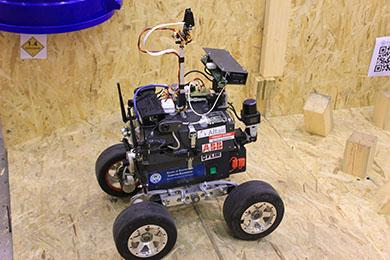
\includegraphics[scale=1.5]{images/pandora_robot.jpg}
  \caption{\small The PANDORA robot of 2014}
  \label{fig:pandora_robot}
\end{figure}

\begin{figure}[H]\centering
  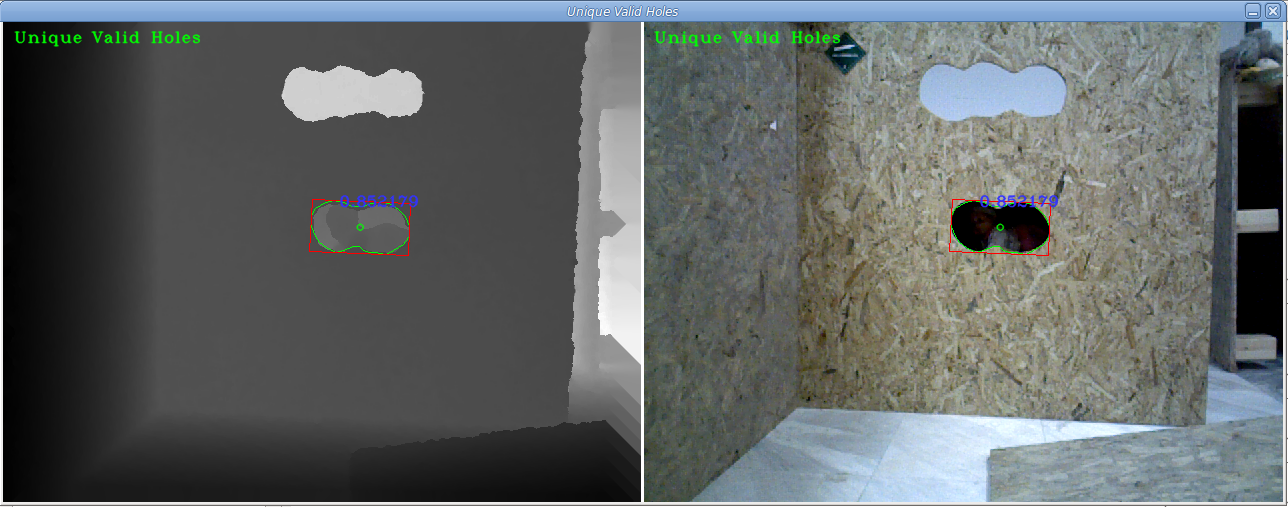
\includegraphics[scale=0.35]{images/unique_holes.png}
  \caption{\small Although the wall has two holes, only the one closer to the
           ground is valid: the one above it is a through hole and
           therefore cannot contain possible victims}
  \label{fig:holes}
\end{figure}

\begin{itemize}
  \item Resources / tools involved: OpenCV, C++, ROS hydro, git
\end{itemize}
